\section{Evaluation}
\label{sec:evalution}

\subsection{Evaluation Setup}

\noindent \textbf{Dataset}. Among existing work on affected package identification~\cite{fastxml,lightxml,chronos,vullibminer}, two datasets are frequently used: VeraCode~\cite{fastxml} and VulLib~\cite{vullibminer}. In this work, we choose to use VulLib instead of VeraCode because it is of better quality. The VulLib dataset contains 2,789 Java vulnerabilities collected from GitHub Advisory. Each package name in VulLib is manually verified by security experts from GitHub Advisory~\cite{githubAD}. In contrast, VeraCode is not verified thus it is prone to errors~\footnote{VeraCode does not use explicit package names ecosystems. For example, the affected package of CVE-2014-2059 is ``org.jenkins-ci.main:jenkins-core'' while VeraCode labels it as three packages: ``jenkins'', ``openshift-origin-cartridge-jenkins'', and ``jenkins-plugin-openshift''}.
% \xueqing{add footnote to explain}.
Since VulLib only focuses on Java, we further extend it to JS, Python and Go by collecting the data from GitHub Advisory following a similar workflow as VulLib. 


% In this paper, we evaluate the effectiveness of \detector{} using the GitHub Advisory database, since each vulnerability in GitHub Advisory is manually reviewed and verified by expert maintainers~\cite{githubReview}.
% In GitHub Advisory, the vulnerabilities are classified by the associated Programming languages~\cite{githubAD}, therefore we can construct a list of programming language-focused datasets~\footnote{Specifically, we extend VulLib, a Java dataset proposed by ~\cite{vullibminer} with the same workflow. 
% Our rationale is that with the help of security experts' verification, VulLib addresses the data quality limitation of VeraCode, another dataset proposed by ~\cite{fastxml} and used by FastXML, LightXML, and Chronos.}. 


% Existing ranking approaches (FastXML, LightXML, Chronos) focus on using the dataset collected by ~\cite{fastxml}, while the ground truths in that dataset are not verified and the quality is low. 
% To improve the data quality, ~\cite{vullibminer} proposed a new dataset VulLib, where the ground truths are verified by security experts of the GitHub advisory~\cite{githubReview}.
% However, VulLib is limited to Java.

% In this work, we extend VulLib to all four languages with the same workflow (thus the ground truths are all verified).
% Additionally, in GitHub Advisory, the vulnerabilities are classified by the associated Programming languages~\cite{githubAD}, therefore we can construct a list of programming language-focused datasets. 

% In this paper, we evaluate the effectiveness of \detector{} using the GitHub Advisory database, since each vulnerability in GitHub Advisory is manually reviewed and verified by expert maintainers~\cite{githubReview}. In GitHub Advisory, the vulnerabilities are classified by the associated Programming languages~\cite{githubAD}, therefore we can construct a list of programming language-focused datasets. 

%Our dataset focuses on four widely used programming languages: Java, JavaScript (JS), Python, and Go. 
The statistics of our dataset are listed in Table~\ref{tab: dataset info}. In total, our dataset includes 2,789 Java, 3,193 JS, 2,237 Python, and 1,351 Go vulnerabilities, respectively. To the best of our knowledge, this is the first dataset for identifying vulnerable packages with various programming languages. For each PL, we split the train/validation/test data with the 3:1:1 ratio. The split is in chronological order to simulate a more realistic scenario and to prevent lookahead bias~\cite{lookahead_bias}.

% Our dataset focuses on four widely used programming languages: Java\footnote{For Java, we use VulLib~\cite{vullibminer}, which is expanded from the Java vulnerabilities in GitHub Advisory.}, JavaScript (JS), Python, and Go. The statistics of our dataset are listed in Table~\ref{tab: dataset info}. In total, our dataset includes 2,789 Java, 3,193 JS, 2,237 Python, and 1,351 Go vulnerabilities, respectively. To the best of our knowledge, this is the first dataset for identifying vulnerable packages with various programming languages. For each PL, we split the train/validation/test data with the 3:1:1 ratio. The split is in chronological order to simulate a more realistic scenario and to prevent lookahead bias~\cite{lookahead_bias}.



%In this table, we also include the number of packages in each ecosystem and their average tokens, which both affected the difficulty of generating package names.
% This table shows that there are 45.41\% zero-shot packages (i.e., not affected by vulnerabilities in the training set), and 36.02\% zero-shot vulnerabilities (i.e., affect only zero-shot packages).
% As discussed in Section~\ref{sec: formal}, we divide the testing set, $\mathcal{L}_{test}$ into $\mathcal{L}_{zero}$, and $\mathcal{L}_{full}$, to evaluate the effectiveness of identifying zero-shot and full-shot vulnerable packages.

\begin{table}[t]
\centering
\caption{The Statistics of the GitHub Advisory Dataset}
\label{tab: dataset info}
\begin{threeparttable}
\small
\begin{tabular}{lrrrr}
\toprule
           & Java & JS   & Python & Go   \\
\midrule
\multicolumn{5}{l}{\textit{\#Vulnerabilities:}}     \\
Training   & 1,668 & 1,915 & 1,342   & 810   \\
Validation & 556   & 639   & 447     & 270   \\
Testing    & 565   & 639   & 448     & 271   \\
Total      & 2,789 & 3,193 & 2,237   & 1,351 \\
\midrule
\multicolumn{5}{l}{\textit{\#Unique packages in the dataset:}}    \\
      & 2,095 & 2,335 & 710     & 601   \\ 
\multicolumn{5}{l}{\textit{\#Total packages in their ecosystems:}}    \\
      & 435k & 2,551k & 507k     & 12k   \\ 
\midrule
\multicolumn{5}{l}{\textit{\#Avg. tokens of packages:}}    \\
& 13.44 & 4.56  & 3.96    & 8.24 \\
\bottomrule
\end{tabular}
% \begin{tablenotes}
%     \footnotesize
%     \item We use the Java dataset expanded by VulLibMiner.
% \end{tablenotes}
\end{threeparttable}
\vspace{-0.3cm}
\end{table}


\noindent \textbf{Comparative Methods}. To evaluate the effectiveness of \detector{}, we contrast it with four existing ranking approaches, FastXML~\cite{fastxml}, LightXML~\cite{lightxml}, Chronos~\cite{chronos}, and VulLibMiner~\cite{vullibminer} for comparison.
Recent studies~\cite{chronos, vullibminer} show that they outperform other approaches, such as Bonsai~\cite{khandagale2020bonsai} and ExtremeText~\cite{wydmuch2018no}.

\noindent \textbf{Models in \detector{}}. The models we evaluate for the \detector{} framework include both commercial LLMs, e.g., ChatGPT (gpt-3.5-turbo) and GPT4 (gpt-4-1106-preview), and open-source LLMs, e.g., LLaMa~\cite{llama} and Vicuna~\cite{vicuna}.


We assess open-source LLMs in two scenarios: few-shot in-context learning using 3 examples\
randomly sampled from the training data and supervised fine-tuning using the full training data.
For the open-source LLMs, we use ICL/SFT + RAG + local search, whereas for commercial LLMs, we use RAG + local search only. 
% (\xueqing{Appendix xxx})

% xueqing{Since there are only 3 examples for each language, perhaps you can attach it in appendix. }
% \tianyu{actually, for each case, I randomly sample three examples (not the same ones)}
% \xueqing{explain how the few-shot examples are selected}

% \tianyu{fine-tune a specific model for each programming language}

% design two scenarios for open-source LLMs: evaluating their base models with in-context learning and fine-tuned models.

\noindent \textbf{Evaluation Environments}
Our evaluations are conducted on the system of Ubuntu 18.04. 
We use one Intel(R) Xeon(R) Gold 6248R@3.00GHz CPU, which contains 64 cores and 512GB memory.
We use 8 Tesla A100 PCIe GPUs with 40GB memory for model training and inference. 
In total, our experiments constitute 200 GPU days (32 groups in RQ1 + 68 groups in RQ2, and each group costs 0.25 GPU days across 8 GPUs).


\noindent \textbf{Metrics.}
Following previous work~\cite{vullibminer, fastxml}, we use three metrics for evaluating \detector{} and baselines: Precision@k (i.e. Accuracy@k), Recall@k, and F1@k ($k=1,2,3$).
% We evaluate the effectiveness of generating the names of affected packages through the Top k accuracy of exact matching (i.e., the correct portion of the first package name generated by LLMs).
% This metric is used by our baseline approaches~\cite{fastxml, lightxml, chronos, vullibminer} and is also widely used in generation tasks.
% It is defined as follows:
% \begin{equation*}
%     Accuracy@k(v) = \frac{|prediction_k(v) \cap label(v)|}{min(k, |label(v)|)}
% \end{equation*}
% where $prediction_k(v)$ is the names of Top K output packages and $label(v)$ is the ground truth of affected packages.

% \xueqing{Check whether this setting follows \cite{vullibminer}?}
%That is, exact match between the first generation or ranking output and the ground truth. 

% Our evaluation answers the following four research questions about \detector{}:
% \begin{itemize}
%     \item \textbf{RQ1}: How effectively can \detector{} generate vulnerable package names?
%     \item \textbf{RQ2}: To what extent can our RAG technique and local search algorithm help generate vulnerable packages?
%     \item \textbf{RQ3}: How efficient is \detector{} when compared with ranking approaches?
%     \item \textbf{RQ4}: How much benefit can security practice gain from our approach?
% \end{itemize}



% \subsection*{\textbf{RQ1}: How effectively can \detector{} generate vulnerable package names?}~\label{sec: rq1}
\subsection{Evaluation of \detector{}~\label{sec: trade off}}

In this subsection, we evaluate the effectiveness of \detector{}. We seek to answer the following research question: How does \detector{} compare to existing work on identifying vulnerable packages? 

\begin{table}[t]
\centering
\caption{Precision@1 of \detector{} and Baselines}
\label{tab: baseline cmp}
\small
\begin{threeparttable}
\begin{tabular}{lccccc}
\toprule
Approach     & Java    & JS     & Python & Go  & Avg.   \\
\midrule
\multicolumn{5}{l}{\textit{Ranking-based Non-LLMs:}}               \\
FastXML       & 0.292   & 0.078  & 0.491  & 0.277 & 0.285 \\
LightXML      & 0.450   & 0.146  & 0.529  & 0.494 & 0.405 \\
Chronos       & 0.516   & 0.447  & 0.550  & 0.710 & 0.556 \\
VulLibMiner   & 0.669   & 0.742  & 0.825  & 0.647 & 0.721 \\
\midrule
\multicolumn{5}{l}{\textit{Commercial LLMs:}} &              \\
ChatGPT       & 0.758   & 0.732  & 0.915  & 0.646  & 0.763\\
GPT4          & \textbf{0.783}   & 0.768  & 0.868  & 0.712 & 0.783 \\
\midrule
\multicolumn{5}{l}{\textit{Few-Shot ICL on Open-Source LLMs:}} & \\
LLaMa-7B      & 0.002   & 0.237  & 0.036  & 0.000 & 0.069 \\
LLaMa-13B     & 0.122   & 0.238  & 0.049  & 0.048 & 0.114 \\
Vicuna-7B     & 0.110   & 0.495  & 0.694  & 0.428 & 0.432 \\
Vicuna-13B    & 0.186   & 0.513  & 0.527  & 0.394 & 0.405 \\
\midrule
\multicolumn{5}{l}{\textit{Full SFT on Open-Source LLMs:}} &   \\
LLaMa-7B      & 0.710  & \textbf{0.773}  & 0.924  & 0.716 & 0.781 \\
LLaMa-13B     & 0.720  & 0.765  & 0.904  & 0.775 & 0.791 \\
Vicuna-7B     & 0.697  & 0.768  & 0.929  & 0.782 & 0.794 \\
Vicuna-13B    & 0.710  & \textbf{0.773}  & \textbf{0.935}  & \textbf{0.804} & \textbf{0.806} \\
\bottomrule
\end{tabular}
% \begin{tablenotes}
%     \footnotesize
%     \item We conduct experiments under the same settings: RAG + local search.
% \end{tablenotes}
\end{threeparttable}
\vspace{-0.3cm}
\end{table}

\begin{table}[t]
\centering
\caption{Precision@2,3 of \detector{} and Baselines}
\label{tab: baseline cmp: precision}
\small
\begin{threeparttable}
\begin{tabular}{lccccc}
\toprule
Approach     & Java    & JS     & Python & Go  & Avg.   \\
\midrule
% \multicolumn{5}{l}{\textit{Precision@1:}}               \\
% Chronos     & 0.516    & 0.447 & 0.550  & 0.710 & 0.556   \\
% VulLibMiner & 0.669    & 0.742 & 0.825  & 0.647 & 0.721   \\
% GPT4        & \textbf{0.783}    & 0.768 & 0.868  & 0.712 & 0.783   \\
% Vicuna-13B  & 0.710    & \textbf{0.776} & \textbf{0.935}  & \textbf{0.804} & \textbf{0.806}   \\
% \midrule
\multicolumn{5}{l}{\textit{Precision@2:}} &              \\
Chronos     & 0.673    & 0.598 & 0.554  & \textbf{0.767} & 0.648   \\
VulLibMiner & 0.695    & 0.725 & 0.789  & 0.669 & 0.720   \\
GPT4        & \textbf{0.762}    & 0.752 & 0.851  & 0.692 & 0.764   \\
Vicuna-13B  & 0.722    & \textbf{0.779} & \textbf{0.858}  & 0.747 & \textbf{0.777}   \\
\midrule
\multicolumn{5}{l}{\textit{Precision@3:}} &   \\
Chronos     & 0.741    & 0.648 & 0.569  & 0.781 & 0.685   \\
VulLibMiner & 0.724    & 0.723 & 0.782  & 0.715 & 0.736   \\
GPT4        & \textbf{0.758}    & 0.749 & 0.754  & 0.678 & 0.735   \\
Vicuna-13B  & 0.743    & \textbf{0.776} &\textbf{ 0.841}  & \textbf{0.785} & \textbf{0.786}   \\
\bottomrule
\end{tabular}
\begin{tablenotes}
    \footnotesize
    \item Precision is the same as Accuracy.
\end{tablenotes}
\end{threeparttable}
\vspace{-0.4cm}
\end{table}

\begin{table}[t]
\centering
\caption{Recall@k of \detector{} and Baselines}
\label{tab: baseline cmp: recall}
\small
\begin{threeparttable}
\begin{tabular}{lccccc}
\toprule
Approach     & Java    & JS     & Python & Go  & Avg.   \\
\midrule
\multicolumn{5}{l}{\textit{Recall@1:}}               \\
Chronos     & 0.400    & 0.412 & 0.286  & 0.605 & 0.426   \\
VulLibMiner & 0.520    & 0.709 & 0.499  & 0.544 & 0.568   \\
GPT4        & \textbf{0.596}    & 0.714 & 0.542  & 0.580 & 0.608   \\
Vicuna-13B  & 0.552    & \textbf{0.736} & \textbf{0.621}  & \textbf{0.688} & \textbf{0.649}   \\
\midrule
\multicolumn{5}{l}{\textit{Recall@2:}} &              \\
Chronos     & 0.623    & 0.591 & 0.346  & \textbf{0.778} & 0.585   \\
VulLibMiner & 0.647    & 0.719 & 0.561  & 0.653 & 0.645   \\
GPT4        & \textbf{0.705}    & 0.744 & 0.585  & 0.675 & 0.677   \\
Vicuna-13B  & 0.669    & \textbf{0.771} & 0.622  & 0.733 & \textbf{0.699}   \\
\midrule
\multicolumn{5}{l}{\textit{Recall@3:}} &   \\
Chronos     & 0.722    & 0.645 & 0.392  & 0.605 & 0.591   \\
VulLibMiner & 0.705    & 0.720 & 0.603  & 0.713 & 0.685   \\
GPT4        & \textbf{0.737}    & 0.745 & 0.597  & 0.675 & 0.689   \\
Vicuna-13B  & 0.720    & \textbf{0.773} & \textbf{0.657}  & \textbf{0.782} & \textbf{0.733}   \\
\bottomrule
\end{tabular}
% \begin{tablenotes}
%     \footnotesize
%     \item We conduct experiments under the same settings: RAG + local search.
% \end{tablenotes}
\end{threeparttable}
% \vspace{-0.4cm}
\end{table}

\begin{table}[t]
\centering
\caption{F1@k of \detector{} and Baselines}
\label{tab: baseline cmp: F1}
\small
\begin{threeparttable}
\begin{tabular}{lccccc}
\toprule
Approach     & Java    & JS     & Python & Go  & Avg.   \\
\midrule
\multicolumn{5}{l}{\textit{F1@1:}}               \\
Chronos     & 0.451    & 0.429 & 0.376  & 0.653 & 0.482   \\
VulLibMiner & 0.585    & 0.725 & 0.622  & 0.591 & 0.635   \\
GPT4        & \textbf{0.677}    & 0.740 & 0.667  & 0.639 & 0.684   \\
Vicuna-13B  & 0.621    & \textbf{0.755} & \textbf{0.746}  & \textbf{0.741} & \textbf{0.719}   \\
\midrule
\multicolumn{5}{l}{\textit{F1@2:}} &              \\
Chronos     & 0.647    & 0.594 & 0.426  & \textbf{0.772} & 0.615   \\
VulLibMiner & 0.670    & 0.722 & 0.656  & 0.661 & 0.680   \\
GPT4        & \textbf{0.732}    & 0.748 & 0.693  & 0.683 & 0.718   \\
Vicuna-13B  & 0.694    & \textbf{0.775} & \textbf{0.721}  & 0.740 & \textbf{0.736}   \\
\midrule
\multicolumn{5}{l}{\textit{F1@3:}} &   \\
Chronos     & 0.731    & 0.646 & 0.464  & 0.682 & 0.634   \\
VulLibMiner & 0.714    & 0.721 & 0.681  & 0.714 & 0.710   \\
GPT4        & \textbf{0.747}    & 0.747 & 0.666  & 0.676 & 0.711   \\
Vicuna-13B  & 0.731    & \textbf{0.774} & \textbf{0.738}  & \textbf{0.783} & \textbf{0.759}   \\
\bottomrule
\end{tabular}
% \begin{tablenotes}
%     \footnotesize
%     \item We conduct experiments under the same settings: RAG + local search.
% \end{tablenotes}
\end{threeparttable}
% \vspace{-0.4cm}
\end{table}




\noindent \textbf{Overall Performance: Existing Work vs. \detector{}}. In Table~\ref{tab: baseline cmp}, Table~\ref{tab: baseline cmp: precision}, Table~\ref{tab: baseline cmp: recall}, and Table~\ref{tab: baseline cmp: F1} (Appendix), we compare the performance of \detector{} and baselines. 
From these tables we can observe that for all programming languages, \detector{} achieves substantially higher accuracies compared to existing work. As a result, by leveraging LLMs, \detector{} can effectively generate the names of affected packages with high accuracies. 

Overall, \detector{} using supervised fine-tuning on the Vicuna-13B model has the best performance. Fine-tuning Vicuna-13B even outperforms the larger ChatGPT and GPT4 models on all datasets besides Java. As a result, the knowledge gap of LLMs can be effectively bridged by leveraging supervised fine-tuning. In Table~\ref{tab: p value} of Appendix, we further report statistical significance tests~\cite{ttest} between the overall best-performing generative approach (i.e., \detector{} using Vicuna-13B SFT) and the best-performing existing work (i.e., VulLibMiner~\cite{vullibminer}). The p-values in all tests are smaller than $1e\textit{-}5$.


\noindent \textbf{When Is \detector{} More Advantageous?} From Table~\ref{tab: baseline cmp} observe that the gap between \detector{} Vicuna-13B SFT
%the best-performing \detector{} method 
and the best-performing existing approach for each programming language are 0.041, 0.031, 0.11, and 0.157. By comparing with the data statistics in Table~\ref{tab: dataset info}, we can see that this gap is highly correlated with \emph{\#Unique packages in the dataset} and \emph{\#Total packages in the ecosystem}. In general, \detector{} is less advantageous when the output package name is longer and has a larger token space. 


\begin{figure}[t]
\centering
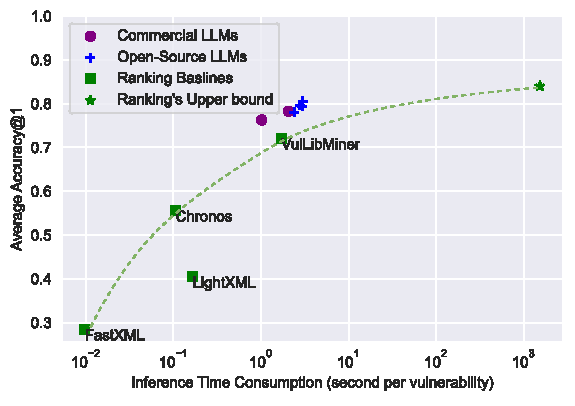
\includegraphics[width=1\linewidth]{figures/efficiency_accuracy_advanced.drawio.pdf}
\caption{Trade-Offs between Efficiency and Accuracy}
\label{fig: efficiency accuracy}
\vspace{-0.3cm}
\end{figure}


% \subsection*{\textbf{RQ3}: How efficient is \detector{} when compared with ranking approaches?}

% In this research question, we evaluate the efficiency of \detector{} when compared with both existing approaches and the estimated upper bound of ranking approaches. 

\noindent \textbf{Efficiency of Existing Work vs. \detector{}}. In Figure~\ref{fig: efficiency accuracy}, we visualize the actual computational cost and accuracy of each method in Table~\ref{tab: baseline cmp}. We further mark the upper bound of the ranking-based approach using LLMs for comparison. The Accuracy@1 is upper-bounded by the recall@512 of TF-IDF, i.e., the best possible Accuracy@1; while the time cost is upper-bounded by the time cost of invoking the 13B model 512 times (10 mins). 


We can observe the \detector{} achieves a sweet spot in the effectiveness and efficiency trade-off. When compared with existing work, \detector{} achieves a better Accuracy@1 while the time cost is comparable to the best-performed existing work~\cite{vullibminer}. When compared with the upper bound, \detector{} achieves a slightly lower Accuracy@1 while consuming less than 1/100 time and computation resources.
%The main reason is that VulLibMiner needs to invoke a lightweight model (BERT) multiple times (e.g., 512) while \detector{} needs to invoke LLMs only once. 

% In Figure~\ref{fig: efficiency accuracy}, additionally, we further mark the upper bound of the existing work for comparison. If we use the larger 13B model in the existing ranking-based approach, the Accuracy@1 is upper-bounded by the recall@512, i.e., assuming that a future model can perfectly order all top-512 packages; whereas the time cost upper-bounded by the time cost of invoking the 13B model 512 times (10 mins). When compared this the upper bound, \detector{} achieves a similar Accuracy@1 while consuming less than 1/100 time and computation resources. As a result, \detector{} achieves a sweet spot in the effectiveness and efficiency tradeoff. 



% \myfindings[1]{\detector{} is highly effective, achieving an average accuracy of 0.790 on four widely-used programming languages while the SOTA approaches achieve only 0.556.}




% \subsection*{\textbf{RQ2}: To what extent can our RAG technique and local search algorithm help generate vulnerable packages?}~\label{sec: rq2}
\subsection{Ablation Studies on \detector{}}
In this subsection, we conduct ablation studies on the three components of \detector{}: supervised fine-tuning, RAG, and local search.
% Additionally, we use Java vulnerabilities to evaluate whether the number and quality of our RAG packages affect the end-to-end effectiveness of \detector{}.

\noindent \textbf{SFT's Improvement}. By comparing the results of in-context learning vs supervised fine-tuning in Table~\ref{tab: baseline cmp}, we can see that SFT outperforms ICL by a larger margin.
%We observe that SFT also outperforms the baseline with neither ICL nor SFT, we have not shown the latter result due to space limit. 
This result indicates that for the 7B and 13B models, supervised fine-tuning on the full training data is essential in bridging the models' knowledge gap. 

% \subsubsection{Methodology}
% We evaluate the effectiveness of \detector{} with various recommended packages to see input augmentation's benefits on \detector{}.
% In this research question, we evaluate the base model of LLaMa-13B without unsupervised fine-tuning because its effectiveness is quite similar to other base models.
% Specifically, we use TF-IDF and VulLibMiner to recommend at most three packages.

\noindent \textbf{RAG's Overall Improvement:}
Table~\ref{tab: rag improvement} shows the improvement of our RAG technique in Accuracy@1.
Specifically, it improves the Accuracy@1 by 9.3\%, 1.8\%, 8.9\%, and 15.7\% on each programming language, respectively.
These improvements indicate that our RAG technique is effective in helping generate the names of vulnerable packages. 
We further report paired t-test results for Table~\ref{tab: rag improvement} in Table~\ref{tab: rag p value} of Appendix. 

Table~\ref{tab: rag improvement} also indicates that RAG's improvement in commercial LLMs is higher than that of open-source LLMs.
Especially in Go vulnerabilities, our RAG technique improves the Accuracy@1 by 57.6\% and 31.0\% on ChatGPT and GPT4.
The main reason is that both ChatGPT and GPT4 do not have sufficient domain knowledge about Go packages as they are relatively newer than packages of other programming languages~\cite{chatgpt_golang}. 
%Thus, RAG can guide these LLMs to generate a proper (existing) package name.

% of our RAG technique in Java vulnerabilities is higher than that in JS, Python, and Go vulnerabilities.
% The major reason is that the names of Java packages are more difficult to generate.
% Even if the improvement in Java is much higher than others, \detector{} still achieves the lowest Accuracy@1 in Java among four programming languages (as shown in Table~\ref{tab: baseline cmp}).

% \noindent \textbf{Difference Among Various Programming Languages}
% Table~\ref{tab: rag improvement} also indicates that the improvement of our RAG technique in Java vulnerabilities is higher than that in JS, Python, and Go vulnerabilities.
% The major reason is that the names of Java packages are more difficult to generate.
% Even if the improvement in Java is much higher than others, \detector{} still achieves the lowest Accuracy@1 in Java among four programming languages (as shown in Table~\ref{tab: baseline cmp}).



\begin{table}[t]
\centering
\small
\caption{RAG's Improvement ($Accuracy@1_{RAG} - Accuracy@1_{Raw}$)}
\label{tab: rag improvement}
\begin{tabular}{lrrrr}
\toprule
\multicolumn{1}{c}{\multirow{1}{*}{Language}} & \multicolumn{1}{c}{Java}                        &        \multicolumn{1}{c}{JS}                 &          \multicolumn{1}{c}{Python}               &     \multicolumn{1}{c}{Go}                    \\
\midrule
\multicolumn{3}{l}{\textit{Commercial LLMs:}}                          &                         &                         \\
ChatGPT                                       & 16.1\% $\uparrow$       & 3.6\% $\uparrow$       & 38.8\% $\uparrow$       & 57.6\% $\uparrow$                \\
GPT4                                          & 12.1\% $\uparrow$       &    0.9\% $\uparrow$                     &      0.9\% $\uparrow$                   &        31.0\% $\uparrow$                 \\ 
\midrule
\multicolumn{5}{l}{\textit{Full SFT on Open-Source LLMs:}}                                                                          \\
LLaMa-7B                                      & 2.2\% $\uparrow$       & 2.2\% $\uparrow$       & 3.1\% $\uparrow$       & 1.8\% $\downarrow$     \\
LLaMa-13B                                     & 3.3\% $\uparrow$       & 0.4\% $\uparrow$       & 2.0\% $\uparrow$       & 3.7\% $\uparrow$       \\
Vicuna-7B                                     & 13.6\% $\uparrow$      & 2.3\% $\uparrow$       & 3.8\% $\uparrow$       & 3.7\% $\uparrow$       \\
Vicuna-13B                                    & 8.7\% $\uparrow$      & 1.2\% $\uparrow$       & 4.9\% $\uparrow$       & 0.0\% -                \\
\midrule
Average                                      & 9.3\% $\uparrow$      & 1.8\% $\uparrow$       & 8.9\% $\uparrow$       & 15.7\% $\uparrow$         \\
\bottomrule
\end{tabular}
\vspace{-0.2cm}
\end{table}



\noindent \textbf{RAG Improvement vs. k/Retrieval Algorithm Choice}. We evaluate whether $k$ and the choice of retrieval algorithm affect the end-to-end effectiveness of \detector{}. Specifically, we focus on Java vulnerabilities (as Java package names are the most difficult to generate). 
The result can be found in Table~\ref{tab: various rag} in our Appendix.

For $k$, we conduct an Analysis of Variance (ANOVA)~\cite{anova} among the Accuracy@1 of six representative numbers of RAG packages (ranging from 1 to 20). Although $k=20$ has a slightly higher accuracy than $k=1$ for both TF-IDF and BERT, this difference is not significant. In fact, the paired t-test results show that there is no significant difference among the Accuracy@1 of different $k$ values ($p=0.814$ for TF-IDF and $p=0.985$ for BERT). 

As for the retrieval algorithm, we observe that Accuracy@1 with TF-IDF results is quite similar to that of non-RAG inputs, and the Accuracy@1 with BERT results is substantially higher than that of non-RAG/TF-IDF results. As a result, it is essential to use BERT-retrieved results in RAG. 


% We show that the Topk F1 scores on the full-shot testing set vary only a little upon different recommended packages.
% For example, the difference between the maximum and minimum values of F1@1 on the full-shot testing set is less than 0.04.
% On the contrary, the recommended packages substantially increase the F1@1 on the zero-shot testing set by 39\% (from 0.394 to 0.547).
% Additionally, recommended packages with higher quality (e.g., from no recommended packages to TF-IDF, or from TF-IDF to VulLibMiner) also help \detector{} to identify zero-shot packages.
% For example, the F1@1 increases by 8\% on average (upon Topk recommended packages) when we use the recommended results from VulLibMiner instead of TF-IDF.
% The main reason for this improvement is that zero-shot packages are difficult for LLMs to identify, and input augmentation provides examples of packages whose functionalities are likely to be affected by a given vulnerability.
% Thus, \detector{} can generate package names from those with similar functionalities instead of all packages.



% \begin{table*}[t]
% \centering
% \scriptsize
% \caption{Accuracy@1 with Various RAG Inputs in Generating the Names of Java Affected Packages}
% \label{tab: various rag}
% \begin{tabular}{llcccccccccccc}
% \toprule
% IR Model:      & None  & \multicolumn{6}{c}{TF-IDF Results}            & \multicolumn{6}{c}{BERT Results}              \\
% \cmidrule(lr){3-8}\cmidrule(lr){9-14}
% \multicolumn{2}{l}{\#RAG packages:} & 1                & 2               & 3     & 5       & 10      & 20      & 1               & 2              & 3     & 5       & 10      & 20      \\
% \midrule
% \multicolumn{3}{l}{\textit{Commercial LLMs:}}                    &                 &       &         &         &         &                 &                &       &         &         &         \\
% ChatGPT    & 0.597 & 0.523 & 0.498 & 0.508 & 0.552 & 0.540 & 0.567 & 0.758 & 0.743 & 0.722 & 0.718 & 0.715 & 0.710 \\
% GPT4       & 0.676 & 0.619 & 0.559 & 0.588 & 0.619 & 0.626 & 0.638 & 0.783 & 0.773 & 0.784 & 0.792 & 0.797 & 0.792 \\
% \midrule
% \multicolumn{5}{l}{\textit{Full SFT on Open-Source LLMs:}}                        &         &         &         &                 &                &       &         &         &         \\
% LLaMa-7B   & 0.688 & 0.692 & 0.697 & 0.701 & 0.563 & 0.591 & 0.609 & 0.710 & 0.701 & 0.710 & 0.678 & 0.665 & 0.683 \\
% LLaMa-13B  & 0.687 & 0.688 & 0.687 & 0.696 & 0.653 & 0.635 & 0.623 & 0.720 & 0.702 & 0.701 & 0.701 & 0.704 & 0.703 \\
% Vicuna-7B  & 0.561 & 0.596 & 0.398 & 0.404 & 0.441 & 0.439 & 0.421 & 0.697 & 0.701 & 0.683 & 0.685 & 0.706 & 0.683 \\
% Vicuna-13B & 0.623 & 0.609 & 0.450 & 0.418 & 0.650 & 0.655 & 0.680 & 0.710 & 0.712 & 0.701 & 0.722 & 0.719 & 0.720 \\
% \bottomrule
% \end{tabular}
% \vspace{-0.4cm}
% \end{table*}

\noindent \textbf{Local Search's Improvement}. 
Table~\ref{tab: post processing} shows the end-to-end 
improvement in Accuracy@1 of \detector{} before and after local search.
Our local search technique improves the Accuracy@1 by 3.43\%, 1.02\%, 1.57\%, and 6.20\% on each programming language. We further report paired t-test results for Table~\ref{tab: post processing} in Table~\ref{tab: local search p value} of Appendix. 

We make the following observations. First, local search is more effective on commercial LLMs (an average improvement of 4.58\%) than fine-tuned open-source LLMs (an average improvement of 2.29\%).
Since commercial LLMs are not fine-tuned, local search plays an important role in improving the effectiveness of generation. Second, local search is more effective on Java and Go than JS and Python. The reason is that since Java and Go packages are longer (8-14 tokens), LLMs are more prone to generating partially correct, non-existing outputs (i.e., Type 2 error in Table~\ref{tab: fault case study}).  Local search can effectively reduce this type of error. 

\begin{table}[t]
\centering
\small
\caption{Local Search's Improvement ($Accuracy@1_{Search} - Accuracy@1_{Raw}$)}
\label{tab: post processing}
\begin{tabular}{lrrrr}
\toprule
\multicolumn{1}{c}{\multirow{1}{*}{Language}} & \multicolumn{1}{c}{Java}                        &        \multicolumn{1}{c}{JS}                 &          \multicolumn{1}{c}{Python}               &     \multicolumn{1}{c}{Go}                    \\
\midrule
\multicolumn{3}{l}{\textit{Commercial LLMs:}}                          &                         &                         \\
ChatGPT                                       & 4.1\% $\uparrow$       & 1.2\% $\uparrow$       & 0.7\% $\uparrow$       & 11.1\% $\uparrow$                \\
GPT4                                          & 5.3\% $\uparrow$       &    2.5\% $\uparrow$                     &      2.9\% $\uparrow$                   &        8.8\% $\uparrow$                 \\ 
\midrule
\multicolumn{5}{l}{\textit{Full SFT on Open-Source LLMs:}}                                           \\
LLaMa-7B                                      & 2.9\% $\uparrow$       & 0.9\% $\uparrow$       & 2.2\% $\uparrow$       & 7.0\% $\uparrow$     \\
LLaMa-13B                                     & 3.3\% $\uparrow$       & 0.3\% $\uparrow$       & 0.7\% $\uparrow$       & 4.1\% $\uparrow$       \\
Vicuna-7B                                     & 3.9\% $\uparrow$      & 0.9\% $\uparrow$       & 1.8\% $\uparrow$       & 3.3\% $\uparrow$       \\
Vicuna-13B                                    & 1.1\% $\uparrow$      & 0.3\% $\uparrow$       & 1.1\% $\uparrow$       & 2.9\% $\uparrow$       \\
\midrule
Average                                      & 3.4\% $\uparrow$      & 1.0\% $\uparrow$       & 1.4\% $\uparrow$       & 6.2\% $\uparrow$         \\
\bottomrule
\end{tabular}
% \vspace{-0.4cm}
\end{table}

% \subsection*{\textbf{RQ3}: How efficient is \detector{} when compared with ranking approaches?}

% In this research question, we evaluate the efficiency of \detector{} when compared with both existing approaches and the estimated upper bound of ranking approaches. 

% \noindent \textbf{Trade-Offs between Effectiveness and Efficiency:}
% It is shown in Figure~\ref{fig: efficiency accuracy}.
% When compared with the SOTA ranking baselines, \detector{} achieves better Accuracy@1  while keeping similar time consumption.
% The main reason is that VulLibMiner needs to invoke a lightweight model (BERT) multiple times (e.g., 512) while \detector{} needs to invoke LLMs only once, thus indicating the effectiveness of replacing ranking with generation.

% Additionally, we also mark the upper bound of ranking approaches for comparison.
% Its time consumption is estimated by invoking Vicuna-13B 512 times, and its Accuracy@1 is estimated as the recall@512 of VulLibMiner, i.e., assuming that a future model can correctly order all candidate packages.
% When compared with the upper bound of ranking approaches, \detector{} achieves similar Accuracy@1 while consuming less than 1/100 time and computation resources.

% \begin{figure}[t]
% \centering
% 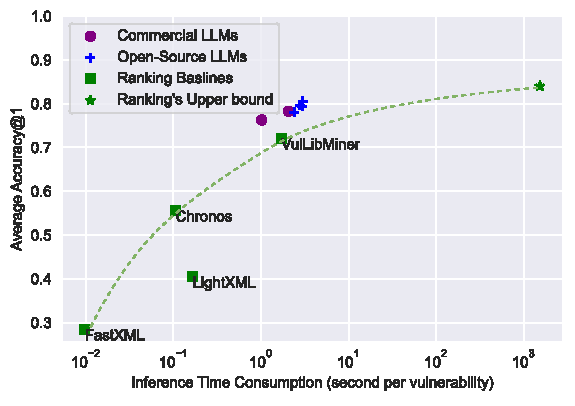
\includegraphics[width=1\linewidth]{figures/efficiency_accuracy_advanced.drawio.pdf}
% \caption{Trade-Offs between Efficiency and Accuracy}
% \label{fig: efficiency accuracy}
% \end{figure}


% \noindent \textbf{The Effectiveness of Constrained Decoding:}
% Table~\ref{tab: post processing} shows the end-to-end Accuracy@1 of \detector{} before and after constrained decoding on open-source LLMs.
% For each combination of programming language and open-source LLMs, constrained decoding improves the end-to-end Accuracy@1 by x.xx\% on average.




% \begin{table}[t]
% \centering
% \small
% \caption{Time Consumption Per Vulnerability}
% \label{tab: time consumption}
% \begin{threeparttable}
% \begin{tabular}{lcccc}
% \toprule
% \multicolumn{1}{c}{\multirow{1}{*}{}} & \multicolumn{1}{c}{\makecell[c]{None}}                        &        \multicolumn{1}{c}{\makecell[c]{Hard\\ Constraints}}                             &     \multicolumn{1}{c}{\makecell[c]{Bigram\\ Constraints}}                    \\
% \midrule
% LLaMa-7B   & 2.41s    & >2h            & 9.48s \\
% LLaMa-13B  & 2.78s    & >2h            & 15.71s \\
% Vicuna-7B  & 2.95s    & >2h            & 9.86s \\
% Vicuna-13B & 3.01s    & >2h            & 15.71s \\
% \midrule
% Average    & 2.79s    & >2h            & 15.71s \\
% \bottomrule
% \end{tabular}
% % \begin{tablenotes}
% %     \footnotesize
% %     \item Column ``All packages'' and ``Top512 packages'' refer to constrained decoding with hard constraints.
% % \end{tablenotes}
% \end{threeparttable}
% \end{table}




% \subsection*{\textbf{RQ4}: How much benefit can security practice gain from our approach?}
% \vspace{-0.2cm}
\subsection{Evaluating \detector{} Performance in Real World Setting}~\label{sec: real world}
% \vspace{-0.4cm}

\noindent To examine \detector{}'s performance in the real-world setting, for each programming language, we randomly sample and report a subset of <vulnerability, affected package> pairs that are not listed in GitHub Advisory (Java: 25, JS: 14, Python: 11, Go: 10). 
We use \detector{} to generate the package names and submit the generated names (\detector{} with Vicuna-13B) to GitHub Advisory. 
% \xueqing{fill xxx with the exact setting in Table 3}. 

At the time of the writing,  the results are summarized below. \textbf{Java}: 21 of them have been accepted and merged into GitHub Advisory. Among the remaining 4 packages, 2 of them are considered non-vulnerabilities, and 2 of them are considered incorrect affected packages. \textbf{JS, Python, and Go}: 13 of them have been accepted and merged into GitHub Advisory (2 JS, 8 Python, 3 Go). The details of these packages are listed in Table~\ref{tab: github issue} of Appendix. 

This result highlights the real-world performance of \detector{} in automatically identifying affected package names. 


% To evaluate \detector{}'s impact on our security practice, we take \detector{} as an oracle to identify <vulnerability, package> pairs as complements of one open-sourced vulnerability database, GitHub Advisory~\cite{githubAD}.
% Note that there are a large amount of Java vulnerabilities besides those included in VulLib and the number of vulnerabilities is rapidly increasing. In this research question, we conduct an empirical study by answering the following two sub-questions:


% \myfindings[4]{\detector{} substantially reduces the manual costs of identifying the affected packages of vulnerabilities.
% Additionally, we demonstrate \detector{}'s high value of security practice by submitting 25 of the identified <vulnerability, package> pairs to GitHub Advisory, and 22 of them are accepted.}


% \begin{table}[t]
% \centering
% \small
% \caption{Constrained Decoding's Improvement in Accracy@1 }
% \label{tab: constrained decoding}
% \begin{tabular}{lcccc}
% \toprule
% \multicolumn{1}{l}{\multirow{1}{*}{Language}} & \multicolumn{1}{c}{Java}                        &        \multicolumn{1}{c}{JS}                 &          \multicolumn{1}{c}{Python}               &     \multicolumn{1}{c}{Go}                    \\
% \midrule
% % \multicolumn{5}{l}{\textit{Existing/non-existing package names:}}                         \\
% %  % & 3.38:1       & 20:1       & 20:1        & 2:1     \\
% % % \midrule
% $\lambda_{LLM}: \lambda_{trie}$ & 5:1       & 20:1       & 20:1        & 5:1     \\
% \midrule
% % LLaMa-7B                         & 2.3\% $\uparrow$      & 0.3\% $\uparrow$       & 1.1\% $\uparrow$       & 2.9\% $\uparrow$       \\
% % LLaMa-13B                         & 2.4\% $\uparrow$      & 0.3\% $\uparrow$       & 1.1\% $\uparrow$       & 2.9\% $\uparrow$       \\
% Vicuna-7B                         & 2.4\% $\uparrow$      & 1.5\% $\downarrow$       & 0.5\% $\uparrow$       & 2.2\% $\uparrow$       \\
% Vicuna-13B                         & 1.9\% $\uparrow$      & 0.1\% $\downarrow$       & 1.1\% $\uparrow$       & 2.9\% $\uparrow$       \\
% \bottomrule
% \end{tabular}
% \end{table}




% \begin{table}[t]
% \centering
% \small
% \caption{Constrained Decoding's Improvement (Accuracy@1)}
% \label{tab: constrained decoding}
% \begin{tabular}{lcccc}
% \toprule
% \multicolumn{1}{c}{\multirow{1}{*}{Language}} & \multicolumn{1}{c}{Java}                        &        \multicolumn{1}{c}{JS}                 &          \multicolumn{1}{c}{Python}               &     \multicolumn{1}{c}{Go}                    \\
% \midrule
% \multicolumn{5}{l}{\textit{Existing/non-existing package names:}}                         \\
%  % & 3.38:1       & 20:1       & 20:1        & 2:1     \\
% % \midrule
% $\lambda_{LLM}: \lambda_{trie}$ & 3:1       & 20:1       & 20:1        & 2:1     \\
% \midrule
% LLaMa-7B                         & 2.25\% $\uparrow$      & 0.3\% $\uparrow$       & 1.1\% $\uparrow$       & 2.9\% $\uparrow$       \\
% LLaMa-13B                         & 2.25\% $\uparrow$      & 0.3\% $\uparrow$       & 1.1\% $\uparrow$       & 2.9\% $\uparrow$       \\
% Vicuna-7B                         & 2.25\% $\uparrow$      & 0.3\% $\uparrow$       & 1.1\% $\uparrow$       & 2.9\% $\uparrow$       \\
% Vicuna-13B                         & 2.25\% $\uparrow$      & 0.3\% $\uparrow$       & 1.1\% $\uparrow$       & 2.9\% $\uparrow$       \\
% \bottomrule
% \end{tabular}
% \end{table}


% \begin{table}[t]
% \centering
% \small
% \caption{Time Consumption of Constrained Decoding per Vulnerability}
% \label{tab: time consumption}
% \begin{threeparttable}
% \begin{tabular}{lcccc}
% \toprule
% \multicolumn{1}{c}{\multirow{1}{*}{}} & \multicolumn{1}{c}{\makecell[c]{None}}                        &        \multicolumn{1}{c}{\makecell[c]{All\\ Packages}}                 &          \multicolumn{1}{c}{\makecell[c]{Top512\\ Packages}}               &     \multicolumn{1}{c}{\makecell[c]{Bigram}}                    \\
% \midrule
% LLaMa-7B   & 2.41s    & >2h          & 81.91s          & 15.71s \\
% LLaMa-13B  & 2.78s    & >2h          & 81.91s          & 15.71s \\
% Vicuna-7B  & 2.78s    & >2h          & 81.91s          & 15.71s \\
% Vicuna-13B & 2.78s    & >2h          & 81.91s          & 15.71s \\
% \midrule
% Average    & 2.78s    & >2h          & 81.91s          & 15.71s \\
% \bottomrule
% \end{tabular}
% \begin{tablenotes}
%     \footnotesize
%     \item Column ``All packages'' and ``Top512 packages'' refer to constrained decoding with hard constraints.
% \end{tablenotes}
% \end{threeparttable}
% \end{table}






% \begin{table*}[t]
% \centering
% \caption{Accuracy@1 with Various Techniques to Address Outputs of Non-Existing Packages}
% \label{tab: post processing}
% \begin{tabular}{lccccccccc}
% \toprule
%            & \multicolumn{3}{c}{Java}                         & \multicolumn{2}{c}{JS}    & \multicolumn{2}{c}{Python} & \multicolumn{2}{c}{Go}    \\
% \cmidrule(lr){2-4}\cmidrule(lr){5-6}\cmidrule(lr){7-8}\cmidrule(lr){9-10}
%            & \makecell[c]{Raw\\ Output} & \makecell[c]{Local\\ Search} & \makecell[c]{Constrained\\ Decoding} & \makecell[c]{Raw\\ Output} & \makecell[c]{Local\\ Search} & \makecell[c]{Raw\\ Output} & \makecell[c]{Local\\ Search} & \makecell[c]{Raw\\ Output} & \makecell[c]{Local\\ Search} \\
% \midrule
% \multicolumn{10}{l}{\textit{Commercial LLMs:}}                                                                                                               \\
% ChatGPT    & 0.717      & 0.758        & -                    & 0.720      & 0.732        & 0.908       & 0.915        & 0.535      & 0.646        \\
% GPT4       & 0.744      & 0.797        & -                    &     0.743       &       0.768       &    0.839         &     0.868         &    0.624        &       0.712       \\
% \midrule
% \multicolumn{10}{l}{\textit{Open-Source LLMs:}}                                                                                                              \\
% LLaMa-7B   & 0.681 & 0.710 & 0.733 & 0.764 & 0.773 & 0.902 & 0.924 & 0.646 & 0.716 \\
% LLaMa-13B  & 0.687 & 0.720 & 0.744 & 0.762 & 0.765 & 0.897 & 0.904 & 0.734 & 0.775 \\
% Vicuna-7B  & 0.658 & 0.697 & 0.721 & 0.759 & 0.768 & 0.911 & 0.929 & 0.749 & 0.782 \\
% Vicuna-13B & 0.699 & 0.710 & 0.729 & 0.770 & 0.773 & 0.924 & 0.935 & 0.775 & 0.804 \\
% \bottomrule
% \end{tabular}
% \end{table*}

